\documentclass{beamer}
\usepackage{biblatex}
\usepackage{tikz}
\usetikzlibrary{positioning}

\title[Lessons Learned after Virtual Lab Design]{%
  Lessons Learned after Virtual Lab Design
}
\author[R. S. D'Souza --- rollen.dsouza@uwaterloo.ca]{%
  Rollen S. D'Souza
}
\date{June 17, 2021}
\addbibresource{references.bib} 
%%%%%%%%%%%%%%%%%%%%%%%%%%%%%%%%%%%%%%%%%%%%%%%%%%%%%%%%%%%%%%%%%%%%%%
%% BEGIN : ECE THEME
%%

% Slide style
\usetheme{Berlin}

% Color Scheme (UW Eng Colours)
\definecolor{UWEngPrimary}{cmyk}{.78,.94,0,0}
\definecolor{UWEngSecondary}{cmyk}{.60,.72,0,0}
\definecolor{UWEngTertiary}{cmyk}{0,0,0,1}

\setbeamercolor{palette primary}{bg=UWEngPrimary}
\setbeamercolor{palette secondary}{bg=UWEngSecondary}
\setbeamercolor{palette tertiary}{bg=UWEngTertiary}
\setbeamercolor{palette quaternary}{%
  fg=UWEngSecondary!5!white!95,%
  bg=UWEngPrimary!5!black!95%
}
\setbeamercolor{background canvas}{bg=UWEngTertiary!5!white!95}
\setbeamertemplate{itemize items}[circle]
\setbeamertemplate{enumerate items}[circle]
\setbeamercolor{itemize item}{fg=UWEngPrimary}
\setbeamercolor{itemize subitem}{fg=UWEngPrimary}
\setbeamercolor{itemize subsubitem}{fg=UWEngPrimary}
\setbeamercolor{item projected}{bg=UWEngPrimary}
\setbeamercolor{subitem projected}{bg=UWEngPrimary}
\setbeamercolor{subsubitem projected}{bg=UWEngPrimary}
%%
%% END   : ECE THEME
%%%%%%%%%%%%%%%%%%%%%%%%%%%%%%%%%%%%%%%%%%%%%%%%%%%%%%%%%%%%%%%%%%%%%%

\begin{document}

\frame{\titlepage}

\section{Background}

\begin{frame}{Traditional Lab Work}
  \emph{Generally accepted wisdom...}
  \begin{center}
    Labs add value by engaging students with the real world aspects of the field and motivate students to learn.
  \end{center}
\end{frame}

\begin{frame}{The Objectives of Laboratory Work}
  Some key goals:~\cite{Feisel2005}
  \begin{itemize}
    \item{
      Instrumentation: learning practical techniques and tools,
    } \pause
    \item{
      Modelling: managing with our imperfect models of reality,
    } \pause
    \item{
      Teamwork and Collaboration: working effectively in teams.
    }
  \end{itemize}
\end{frame}

\section{Going Online}

% \frame<1>[label=goingonline]{
%   \frametitle{Going Online: Meeting the Objectives}
%   How do we meet these objectives?
%   \begin{itemize}
%     \item{
%       \color<2->{UWEngPrimary!50!white!50}
%       Instrumentation and Modelling
%     } \pause
%     \item{
%       Teamwork and Collaboration
%     }
%   \end{itemize}
% }

\begin{frame}{Instrumentation and Modelling}
  \begin{tikzpicture}[x=1cm, y=1cm]
    \node[at={(0,0)}, anchor=south west]{
      \includegraphics{InstrumentModelling.pdf}
    };
    \node[at={(5, 3)}, anchor=south west]{
      \begin{minipage}{5cm}
      \begin{itemize}
        \item{
          \color<2->{UWEngPrimary!50!white!50}
          Instrumentation skills are hard to replicate in remote or virtual labs.
        }
        \item{
          \color<2->{UWEngPrimary!50!white!50}
          What software instrumentation will students have to use in the future?
        }
      \end{itemize}
      \end{minipage}
    };
    \node<2->[at={(5, 0)}, anchor=south west]{
      \begin{minipage}{5cm}
      \begin{itemize}
        \item{
          Can record the real world, or use simulation.
        }
        \item{
          Virtual models (simulations) can be too perfect.~\cite{Chen2010}
        }
      \end{itemize}
      \end{minipage}
    };
    \node[at={(0, 0)}, anchor=south west]{
      \fontsize{0.1cm}{0.12cm}\selectfont
      Graphics created by rawpixel.com and brgfx --- \href{https://www.freepik.com/vectors/icons}{freepik.com}
    };
  \end{tikzpicture}
\end{frame}

\begin{frame}{Model Interaction}
  \begin{center}
  \begin{tikzpicture}
    \node[] (Coarse) {%
      \begin{minipage}{5.5em}
        \begin{center}No Model\end{center}
      \end{minipage}%
    };
    \node[right={6cm of Coarse}] (Fine) {%
      \begin{minipage}{5.5em}
        \begin{center}Real World\end{center}
      \end{minipage}%
    };
    \node[right={2cm of Coarse}] (StudentModel) {};
    \node[right={4cm of Coarse}] (InstructorModel) {};
    \node[above={2em of InstructorModel}] (InstructorText) {};
    \node[above={2em of InstructorModel}] {
      \includegraphics[scale=0.25]{SpaceShuttle_Trans.png}
    };

    \draw[<->] (Coarse.east) -- (Fine.west);
    \fill (StudentModel.base) circle[radius=0.05cm];
    \fill (InstructorModel.base) circle[radius=0.05cm];

    \node[below={2em of StudentModel}] (StudentText) {
      Student's Model
    };
    \draw[->] (StudentText.north) -- (StudentModel.south);

    \node[below={0.5em of Fine.south east}, anchor={north east}] (Rover) {
      \includegraphics[scale=0.10]{roveroverlook.jpg}
    };
    \node[anchor={south west}, at={(Rover.south west)}] {
      \fontsize{0.1cm}{0.12cm}\selectfont
      \color{white}
      Credits: NASA/JPL-Caltech/ASU/MSSS
    };

    \node[at={(InstructorText)}] (InstructorTextBox) {
      Simulated Model
    };
    \draw[->] (InstructorTextBox.south) -- (InstructorModel.north);
  \end{tikzpicture}
  \end{center}
  \pause
  if done well students can experience ``real world'' effects~\cite{Chen2010};
  can be hard to implement well~\cite{Waestberg2019}.
\end{frame}

% \againframe<3>{goingonline}

\begin{frame}{Collaboration in Person}
  \begin{center}
    \includegraphics[page=1]{ThoughtExperiment.pdf}
  \end{center}
\end{frame}

\begin{frame}{Collaboration Online}
  \begin{center}
    \begin{tikzpicture}
      \node[at={(0,0)}, anchor={south west}] {
        \includegraphics[page=2]{ThoughtExperiment.pdf}
      };

      \node[at={(0,0)}, anchor={south west}] {
        \begin{minipage}{4cm}
          Peer-to-peer social presence is important.\\
          Can affect learning~\cite{Fiock2020}.\hfill
        \end{minipage}
      };
    \end{tikzpicture}
  \end{center}
\end{frame}

\section{Ending Thoughts}

\begin{frame}{Lessons as we go back in person...}
  %Implementing virtual content was hard.
  We have implemented one year of virtual content.
  \pause
  Opportunity to consider blended content that can produce better student learning outcomes~\cite{Bumbacher2017, Olympiou2011}.
  \pause
  \begin{itemize}
    \item{
      Are we incorporating modern instrumentation as well as we could?
    }
    \item{
      Can we leverage our newly developed virtual/remote content?
    }
    \item{
      Do we take as seriously the intergroup collaboration as we do intragroup collaboration?
    }
  \end{itemize}
\end{frame}

\section{Appendix}

\begin{frame}
  \vfill
  \centering
  \begin{beamercolorbox}[sep=8pt,center,shadow=false,rounded=false]{title}
    \usebeamerfont{title}\insertsectionhead\par%
  \end{beamercolorbox}
  \vfill
\end{frame}

\begin{frame}{Model Interaction}
  \begin{center}
  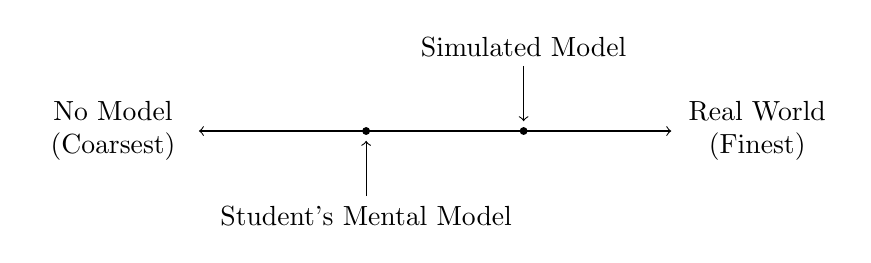
\begin{tikzpicture}
    \node[] (Coarse) {%
      \begin{minipage}{5.5em}
        \begin{center}No Model\\(Coarsest)\end{center}
      \end{minipage}%
    };
    \node[right={6cm of Coarse}] (Fine) {%
      \begin{minipage}{5.5em}
        \begin{center}Real World\\(Finest)\end{center}
      \end{minipage}%
    };
    \node[right={2cm of Coarse}] (StudentModel) {};
    \node[right={4cm of Coarse}] (InstructorModel) {};

    \draw[<->] (Coarse.east) -- (Fine.west);
    \fill (StudentModel.base) circle[radius=0.05cm];
    \fill (InstructorModel.base) circle[radius=0.05cm];

    \node[below={2em of StudentModel}] (StudentText) {
      Student's Mental Model
    };
    \draw[->] (StudentText.north) -- (StudentModel.south);
    \node[above={2em of InstructorModel}] (InstructorText) {
      Simulated Model
    };
    \draw[->] (InstructorText.south) -- (InstructorModel.north);
  \end{tikzpicture}
  \end{center}
  \begin{itemize}
    \item{
      if done well students can perform the lab while still experiencing ``real world'' effects~\cite{Chen2010}.
    }
    \item{
      Powerful; can consider scenarios not possible in a physical lab but exists in the real-world.
    }
    \item{
      This can be difficult to implement; must consider human resources available~\cite{Waestberg2019}.
    }
  \end{itemize}
\end{frame}

\renewcommand*{\bibfont}{\tiny}
\begin{frame}{References}{}
\printbibliography[heading=none]
\end{frame}


\end{document}